\subsection{CFD-DEM Model}
\begin{frame}{Particle in Fluid Field}
% \begin{figure}
% 	\centering
% 	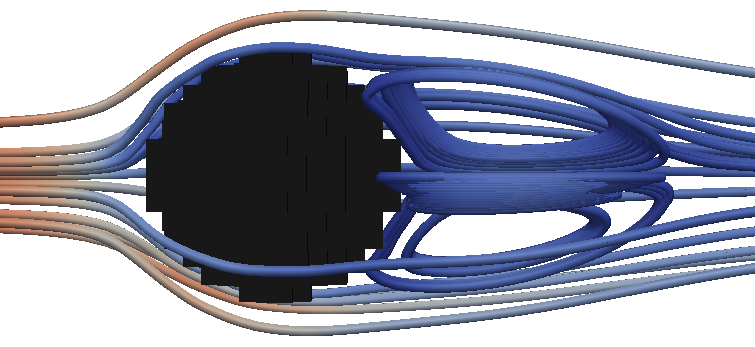
\includegraphics[width=0.5\linewidth]{chapters/figures/single-sphere-drag} 
% 	\caption{Streamlines around a single sphere in $Re = 100$ flow.}
% 	\label{fig:fluid-around-particle}
% \end{figure}

Add a drag on particle due to passing fluid and energy exchange at the interface. Eqs.~\ref{eq:newtons-second} and~\ref{eq:thermoFirstLaw} become,
\begin{subequations}\label{eq:cfdem-dem-momentum}
\begin{align}
	m_i  \ddt{\vec{r}_i}  &= m_i\vec{g} + \sum_{j=1}^{Z} \vec{f}_{n,ij} + \beta_i V_i \Delta \vec{u}_{if}\\
	m_iC_i \ddt{T_i} &= Q_{s,i} + \sum_{j=1}^Z Q_{ij} + \beta_{E,i} A_i \Delta T_{if}
\end{align}
\end{subequations}
the inter-phase exchange coefficients are defined as
\begin{subequations}
\begin{align}
	\beta_{i} &= \frac{18\mu_f}{d_{p,i}^2}(1-\phi_k)\phi_k F\\
	\beta_{E,i} &= \frac{\Nu k_f}{d_{p,i}}
\end{align}
\end{subequations}

\end{frame}


\begin{frame}{Non-dimensional Drag Correlations}
Koch, Hill, \& Ladd provide non-dimensional drag as
\begin{equation}\label{eq:khl-correlation}
	F = F_0(\phi) + F_3(\phi)\Re
\end{equation}
where 
\begin{subequations}
\begin{align}
F_0 &= \begin{cases}
	\frac{1+3(\phi/2)^{1/2} + (135/64)\phi\ln\phi + 16.14\phi}{1 + 0.681\phi - 8.48 \phi^2 + 8.16\phi^3} & \text{if $\phi < 0.4$}\\
	10.0\,\frac{\phi}{(1-\phi)^3} & \text{if $\phi > 0.4$} 
	\end{cases}\\
F_3 &= 0.0673 + 0.212\phi + 0.0232 \frac{1}{(1-\phi)^5}
\end{align}
\end{subequations}

Li \& Mason provide Nusselt number as
\begin{equation}\label{eq:li-mason-correlation}
	\Nu = \begin{cases}
	2+ 0.6\epsilon^n\Re_p^{1/2}\Pr^{1/3} 										& \Re_p < 200\\
	2+ 0.5\epsilon^n\Re_p^{1/2}\Pr^{1/3} + 0.02 \epsilon^n \Re_p^{0.8}\Pr^{1/3} & 200 < \Re_p < 1500\\
	2+ 0.000045\epsilon^n\Re_p^{1/2}			 								& \Re_p > 1500
	\end{cases}
\end{equation}
where they found from experiments that $n=3.5$ was appropriate for 3~mm polymer pellets in dilute flows
\end{frame}


\begin{frame}{Fluid Conservation Equations}
Volume-averaged Navier-Stokes and Energy equations with closure terms from DEM data,
\begin{subequations}\label{eq:cfd-equations}
\begin{align}
\pder[\epsilon_k \rho_f]{t} + \nabla\cdot(\epsilon_k \vec{u}_f \rho_f) &= 0\\
\pder[\epsilon_k \vec{u}_f]{t} + \nabla\cdot(\epsilon_k \vec{u}_f \vec{u}_f) &= -\frac{\epsilon_k}{\rho_f}\nabla P_f + \nabla\cdot\left(\nu_f\epsilon_k\nabla \vec{u}_f\right) - \frac{\vec{S}_k}{\rho_f}\\
\pder[\epsilon_k T_f]{t} + \nabla\cdot(\epsilon_k \vec{u}_f T_f) &= \nabla\left(\epsilon_k\nabla T_f\right)-\frac{E_k}{\rho_fC_f}
\end{align}
\end{subequations}

Coupling the fluid phase to the particles happens with the sink terms in momentum and energy of $\vec{S}_k$ and $E_k$
\begin{subequations}\label{eq:cfd-sources}
\begin{align}
	\phi_k &= 1- \epsilon_k = \frac{1}{V_k}\sum_{\forall i \in k} V_{p,i}\\
	\vec{S}_k &= \frac{1}{V_k}\sum_{\forall i \in k} \beta_i V_i \Delta \vec{u}_{if} \label{eq:cfd-mom-source}\\
	E_k &= \frac{1}{V_k}\sum_{\forall i \in k} \beta_{E,i} A_i \Delta T_{if}
\end{align}
\end{subequations}
\end{frame}

\begin{frame}{Lagrangian-Eulerian Mapping}
\begin{figure}[t]
	\centering
	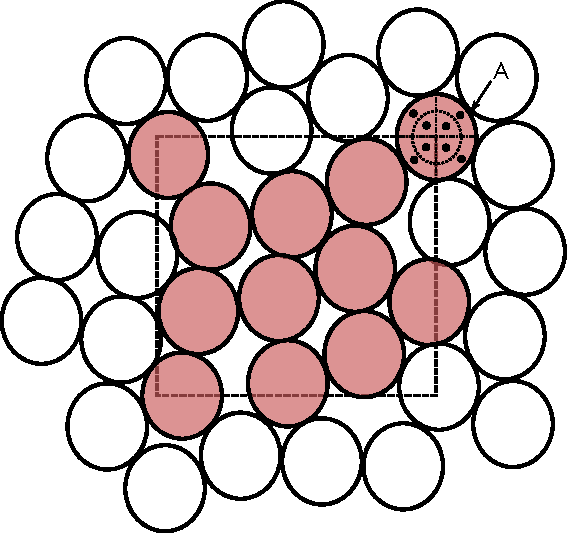
\includegraphics[width=0.5\linewidth]{chapters/figures/void-fraction-divided-cell.pdf}\label{fig:centroid-void-fraction-divided}
	\caption{The dashed line represents a computational cell in which exist many particles. The particles with centroids inside the cell are shaded red.}
\end{figure}
\begin{equation}
	\epsilon_\text{cell} = 1-\frac{1}{V_\text{cell}}\sum_{i = A}^{i=L}w_iV_{p,i}
\end{equation}
\end{frame}